% !TEX root = main.tex

\section{神经网络}
\subsection{感知机与单层神经网络}
下图是M-P神经元(neuron)模型[McCulloch and Pitts, 1943],一直沿用至今。
\begin{figure}[H]
\centering
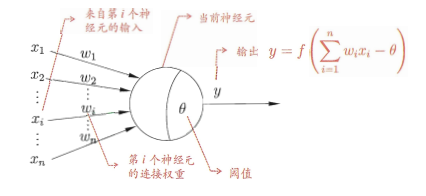
\includegraphics[width=0.6\linewidth]{fig/MP-neuron.png}
\end{figure}

感知机(perceptron)由两层神经元组成,输入层接收外界输入信号后传递给输出层,输出层是M-P神经元,亦称``阈值逻辑单元''(threshold logic unit)。
\begin{figure}[H]
\centering
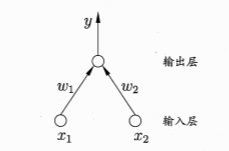
\includegraphics[width=0.4\linewidth]{fig/perceptron.png}
\end{figure}

感知机能够容易实现与或非运算,只要设定好特定的权重和阈值。

感知机的学习规则非常简单,对训练样例$(\vx,y)$,如果当前感知机的输出为$\hat{y}$,则感知机的权重依照下式修改
\[\begin{aligned}
w_i&\gets w_i+\Delta w_i\\
w_i&= \eta(y-\hat{y})x_i
\end{aligned}\]
其中$\eta\in(0,1)$称为学习率(learning rate)。
感知机预测正确则不发生变化,否则根据错误的程度对权重进行修改。

Minsky和Papert[1969]证明了若两类模式是线性可分的,则必然存在一个线性超平面将它们分开,感知机一定收敛;但非线性可分,如异或,感知机无法收敛。
\begin{figure}[H]
\centering
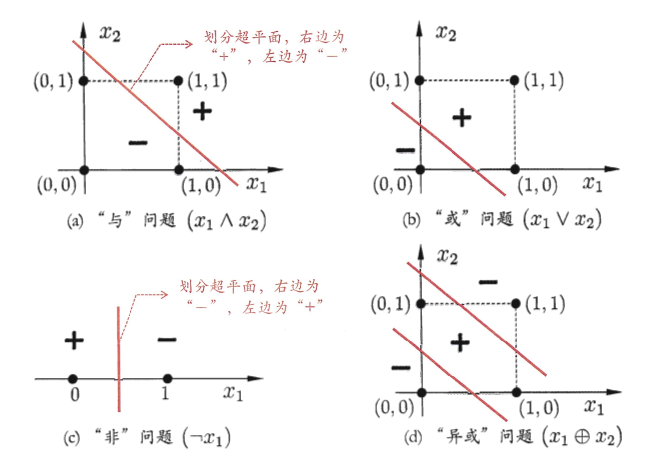
\includegraphics[width=0.7\linewidth]{fig/linear-separable.png}
\end{figure}

\subsection{多层神经网络}
要解决非线性可分问题,则需要用到多层神经网络。
\begin{figure}[H]
\centering
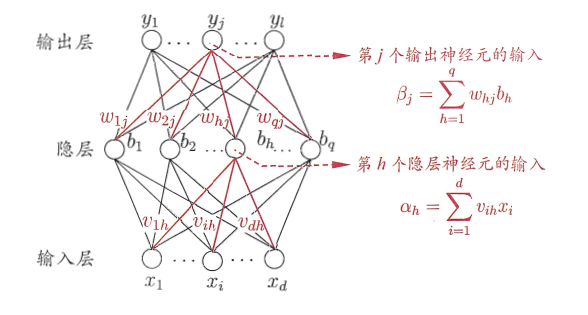
\includegraphics[width=0.6\linewidth]{fig/BP.png}
\end{figure}

用反向传播算法(Back propagation, BP)进行学习。

通用近似定理[Hornik, 1989]证明,只需一个包含足够多神经元的隐层,多层前馈神经网络就能以任意精度逼近任意复杂度的连续函数。
然而,如何设置神经元的个数却没有固定的标准。

\subsection{深度学习}
一般情况下,复杂模型的训练效率低,易陷入过拟合,因此难以受到人们青睐。
但是随着云计算和大数据时代的到来,计算能力的大幅提高可以有效缓解训练的低效性,训练数据的大幅增加则可以降低过拟合风险,因此以深度学习(deep learning)为代表的复杂模型开始受到人们关注。

\begin{itemize}
	\item 深度信念网络(Deep belief network, DBN)[Hinton, 2006]:每一层都是一个受限Boltzmann机
	\item 卷积神经网络(Convolutional neural network, CNN)[LeCun, 1995]:权值共享
\begin{figure}[H]
\centering
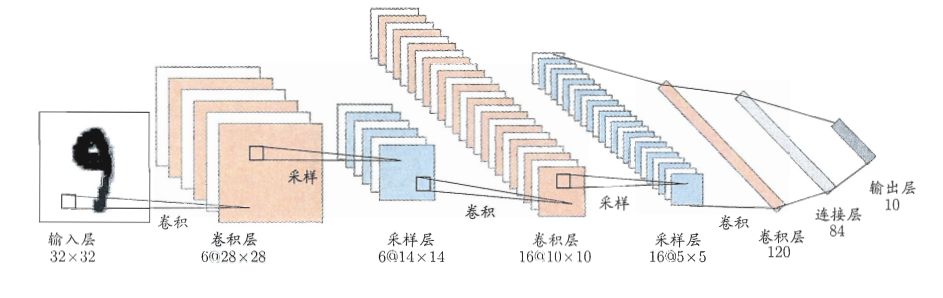
\includegraphics[width=0.8\linewidth]{fig/LeNet.png}
\end{figure}
\end{itemize}

深度学习实际上是通过多层处理,将初始的``低层''特征表示转化为``高层''特征表示后,用``简单的模型''就可以完成复杂的学习任务。(网络前若干层都是在特征表示,最后一层则是简单的分类。)
因此可以将深度学习理解为进行特征学习或表示学习(representation learning)。

以往机器学习在用于现实任务时,描述样本的特征通常需要人类专家进行设计,这称为特征工程(feature engineering)。
但现在有了深度学习,则是进一步将特征提取的工作交由机器来做。

\begin{itemize}
\item 局部最优
\item 梯度消失:ReLU、ResNet
\item 过拟合:正则化(Dropout、早停)
\item 优化:适应性学习率(Momentum、Nesterov、Adagrad、Adadelta、RMSprop、Adam)
\end{itemize}

\subsection{Transformer}
\begin{quote}
Vaswani et al., \emph{Attention Is All You Need}, NeurIPS, 2017
\end{quote}

\begin{figure}[H]
\centering
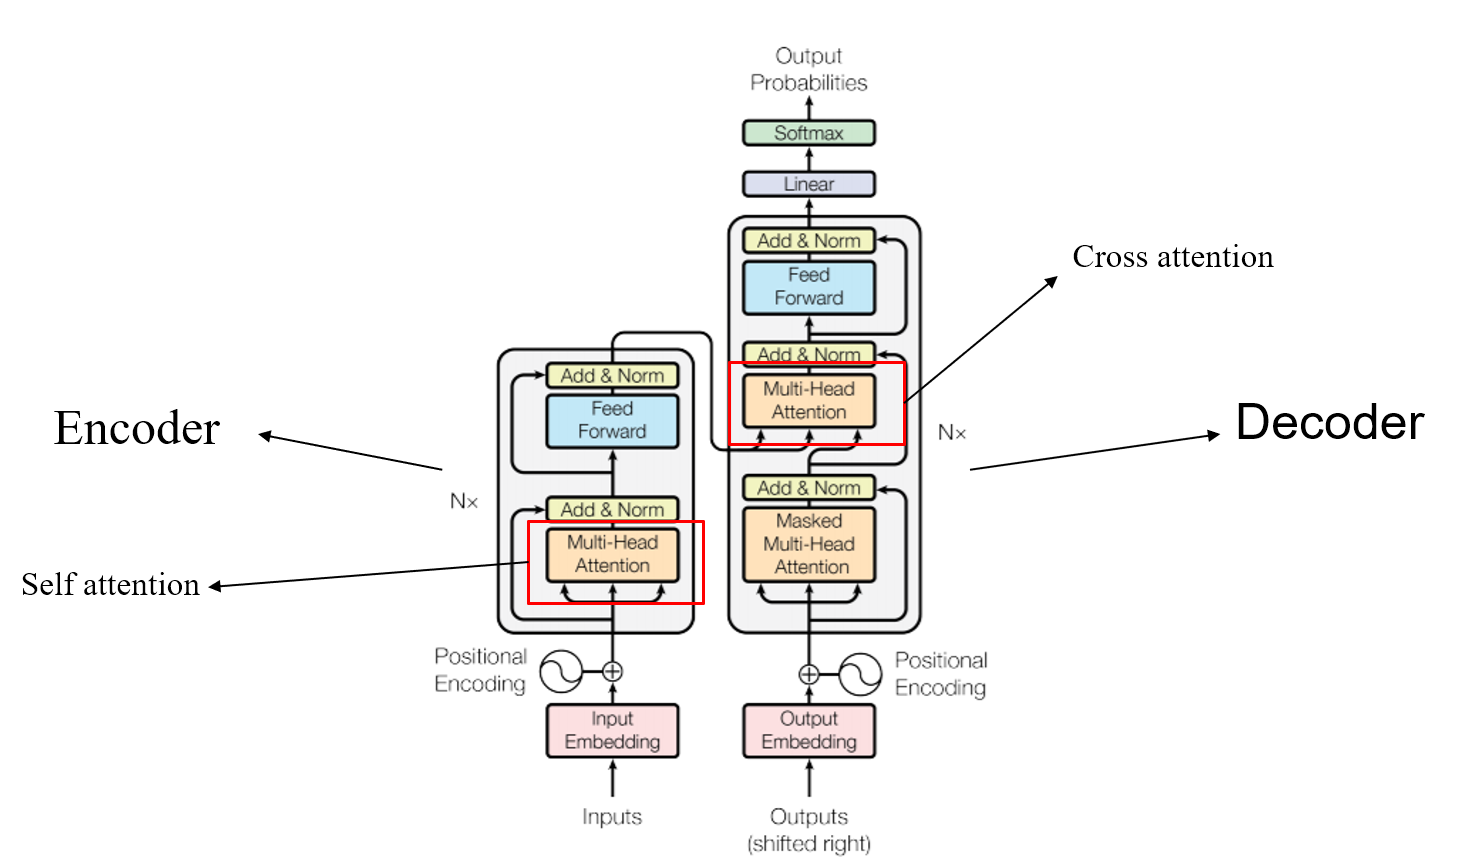
\includegraphics[width=0.8\linewidth]{fig/transformer.png}
\end{figure}
\begin{figure}[H]
\centering
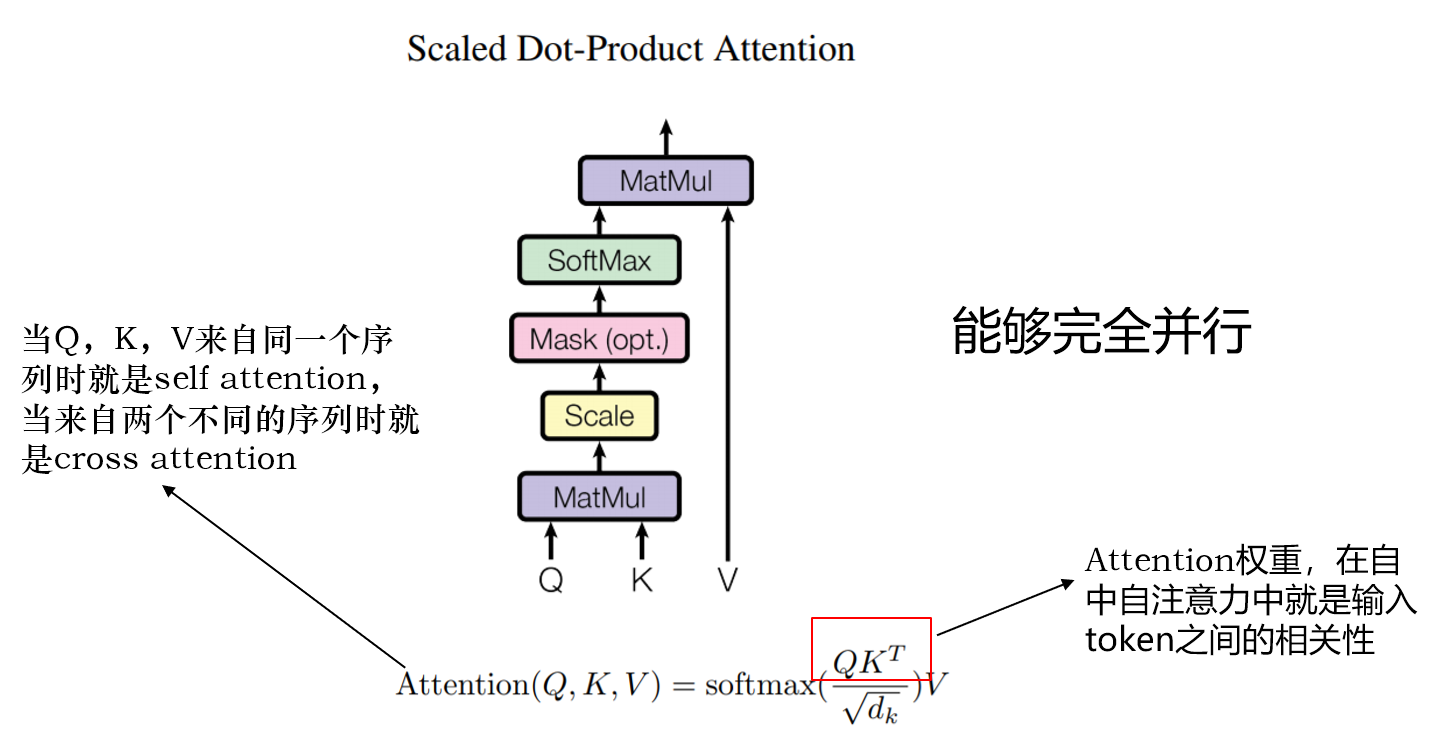
\includegraphics[width=0.8\linewidth]{fig/attention.png}
\end{figure}
\begin{figure}[H]
\centering
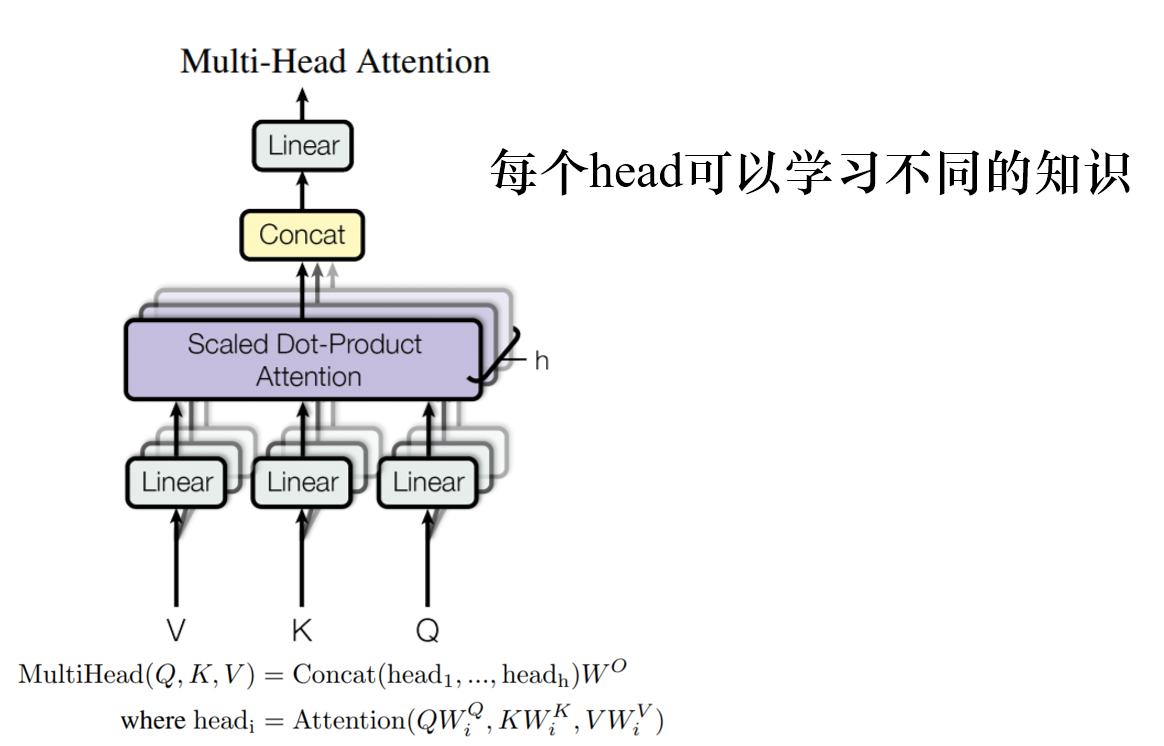
\includegraphics[width=0.6\linewidth]{fig/multihead.png}
\end{figure}

进而有BERT模型
\begin{figure}[H]
\centering
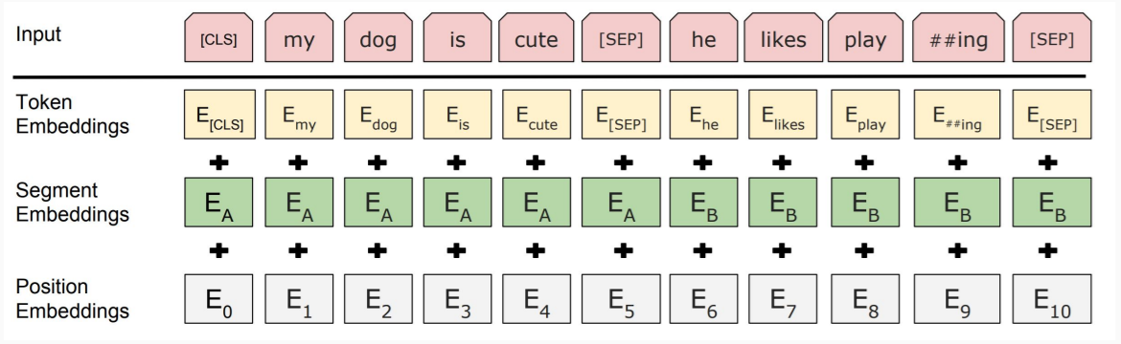
\includegraphics[width=0.8\linewidth]{fig/bert.png}
\end{figure}

\subsection{神经网络的历史发展}
\begin{itemize}
	\item 1940s:M-P神经元模型
	\item 1950s:感知机
	\item 1969:Minsky(MIT)出版了《感知机》一书,指出单层神经网络无法解决非线性问题,而多层神经网络训练算法看不到希望,直接导致神经网络研究进入了``冰河期''
	\item 1974:Werbos(Harvard)发明BP算法,但仍处于冰河期不受重视
	\item 1983:Hopfield(Caltech)利用神经网络在旅行商问题(TSP)上取得当时最好结果,后来Rumelhart等人重新发明BP算法,掀起神经网络第二次高潮
	\item 1990s:统计学习理论和支持向量机的兴起,神经网络学习的理论性质不够清楚、试错性强、使用中充斥大量窍门的弱点更为明显,神经网络研究又陷入低谷
	\item 2010s:算力提升+大数据涌现,神经网络在ImageNet上以绝对优势夺冠,神经网络迎来第三次高潮
\end{itemize}